\chapter{Factory Method}
\section{Intento}

Definisce un'interfaccia per la creazione di un oggetto, ma lasciare che le sottoclassi decidano quale classe istanziare.

(come l'Abstract Factory ma con un solo Product)


%---
\section{Struttura}

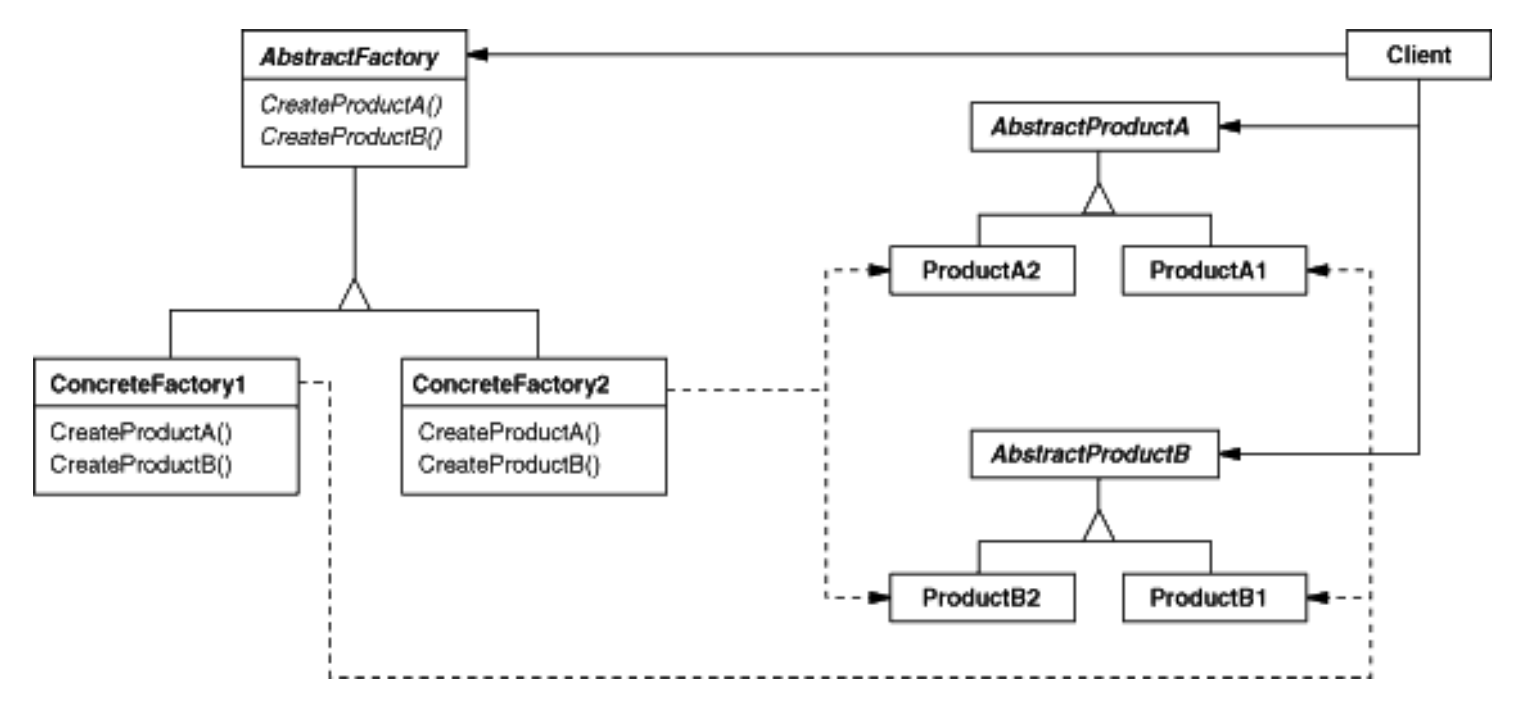
\includegraphics[width=\textwidth]{/Users/matt/Documents/LaTex/Design Pattern LaTex/FactoryMethod/Structure1}


%---
\section{Implementazione}

\subsection{Due varietà principali.}
Le varianti del modello Factory Method sono

\begin{enumerate}
    \item il caso in cui la classe Creator è una classe astratta e non fornisce un'implementazione per il Factory Method che dichiara.

    Questo caso richiede sottoclassi per definire un'implementazione, perché non esiste un valore predefinito ragionevole. Si aggira il dilemma di dover istanziare classi imprevedibili.

    \item il caso in cui Creator è una classe concreta e fornisce un'implementazione predefinita per il Factory Method. È anche possibile avere una classe astratta che definisce un'implementazione predefinita, ma è meno comune.

    Perciò il Creator concreto utilizza il Factory Method principalmente per la flessibilità. Sta seguendo una regola che dice "Crea oggetti in un'operazione separata in modo che le sottoclassi possano sovrascrivere il modo in cui sono state create". Questa regola garantisce che i progettisti di sottoclassi possano modificare la classe di oggetti istanziati dalla loro classe genitore, se necessario.

\end{enumerate}

\subsection{Factory Method parametrizzati.}
Un'altra variazione sul modello consente al Factory Method di creare più tipi di Product. Il Factory Method accetta un parametro che identifica il tipo di oggetto da creare. Tutti gli oggetti creati dal Factory Method condivideranno l'interfaccia del prodotto.

Un metodo di fabbrica parametrizzato ha la seguente forma generale, dove MyProduct e YourProduct sono sottoclassi di Product:

\begin{lstlisting}[language=c++]
    class Creator {
        abstract Product Create(ProductId);
    };

    Product Create (ProductId id) {
        if (id == MINE) {
            return new MyProduct;
        }

        if (id == YOURS) {
            return new YourProduct;
            // repeat for remaining products...
        }

        return 0; 
    }
\end{lstlisting}

L'override di un Factory Method parametrizzato consente di estendere o modificare in modo semplice e selettivo i prodotti prodotti da un Creator. Puoi introdurre nuovi identificatori per nuovi tipi di prodotti oppure puoi associare identificatori esistenti a prodotti diversi.
Ad esempio, una sottoclasse MyCreator potrebbe scambiare MyProduct e YourProduct e supportare una nuova sottoclasse TheirProduct:

\begin{lstlisting}[language=c++]
    Product Create (ProductId id) {
        if (id == YOURS) {
            return new MyProduct;
        }
        
        if (id == MINE) {
            return new YourProduct;
            // N.B.: switched YOURS and MINE
        }

        if (id == THEIRS) {
            return new TheirProduct;
        }

        return Create(id); // called if all others fail
    }
\end{lstlisting}

Nota che l'ultima cosa che fa questa operazione è chiamare Create sulla classe genitore. Questo perché Create gestisce solo My, Your e Their in modo diverso rispetto alla classe genitore. Non è interessato ad altre classi. Quindi MyCreator estende i tipi di prodotti creati e rinvia la responsabilità della creazione di tutti i prodotti tranne alcuni al suo genitore.

\subsection{Utilizzo di modelli per evitare la sottoclasse.} 
Come abbiamo detto, un altro potenziale problema con i Factory Method è che potrebbero costringerti a sottoclassi solo per creare gli oggetti Product appropriati. Un altro modo, in C++, è fornire una sottoclasse di template di Creator parametrizzata dalla classe Product:

\begin{lstlisting}[language=c++]
    class Creator {
        abstract Product CreateProduct() = 0;
    };

    templateclass <class TheProduct>

    class StandardCreator: public Creator {
        public:
            virtual Product* CreateProduct();
    };


    template <class TheProduct>

    Product* StandardCreator<TheProduct>::CreateProduct () {
    return new TheProduct;
    }
\end{lstlisting}

Con questo modello, il client fornisce solo la classe di prodotto, non è richiesta alcuna sottoclasse di Creator.

\begin{lstlisting}[language=c++]
class MyProduct : public Product {
    public:
        MyProduct();
        // ... 
};

StandardCreator<MyProduct> myCreator;
\end{lstlisting}


%---
\section{Esempio Java}
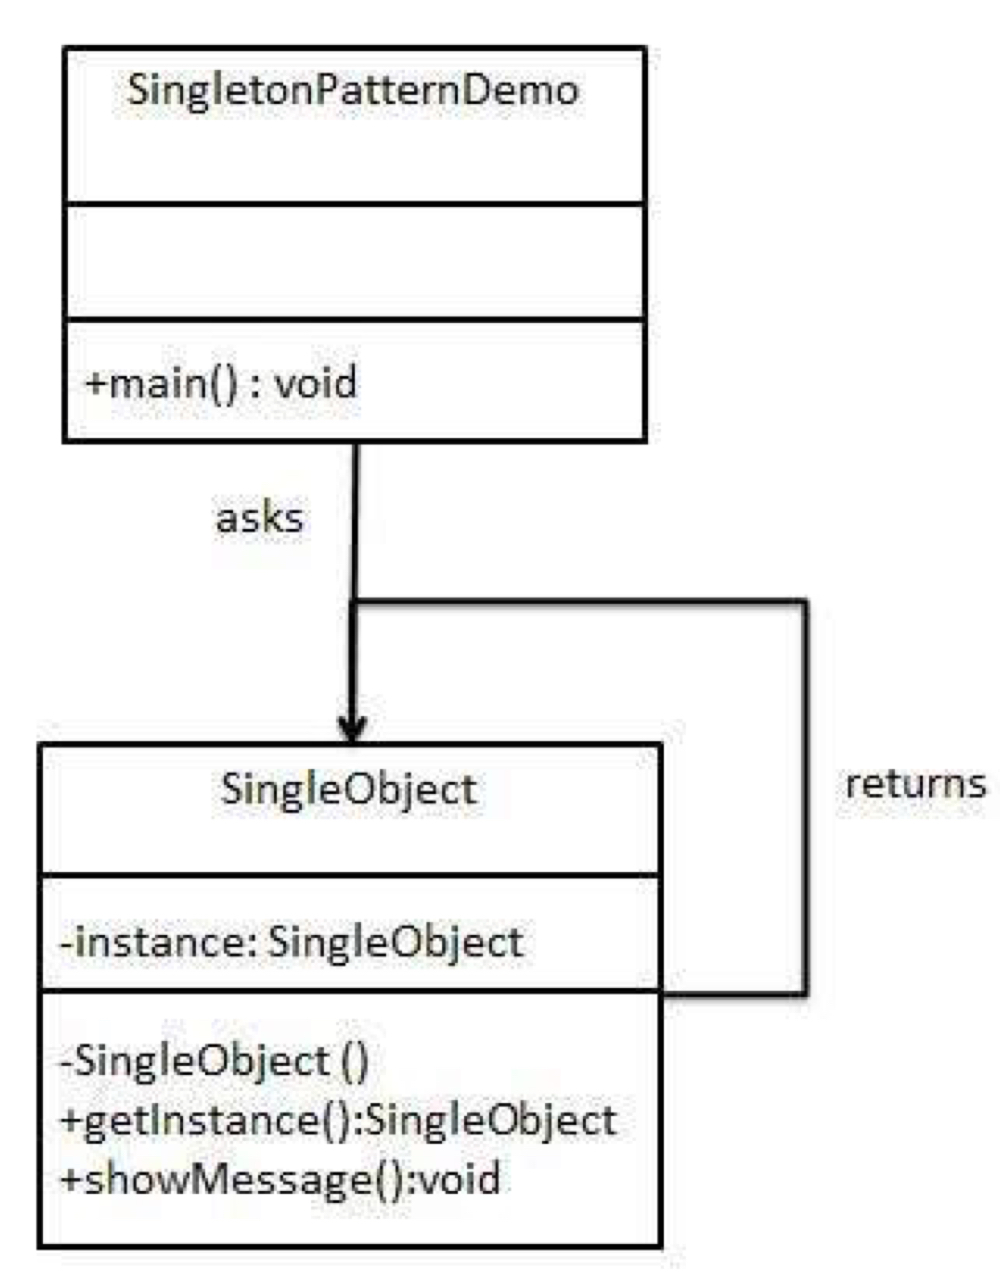
\includegraphics[width=\textwidth]{/Users/matt/Documents/LaTex/Design Pattern LaTex/FactoryMethod/Example1}

\subsection{Circle.java}
\begin{lstlisting}[language=java]
    public class Circle implements Shape {

        @Override
        public void draw() {
            System.out.println("CERCHIO");
        }
        
    }
\end{lstlisting}

\subsection{Rectangle.java}
\begin{lstlisting}[language=java]
    public class Rectangle implements Shape {

        @Override
        public void draw() {
            System.out.println("RECTANGLE");
        }
        
    }
\end{lstlisting}

\subsection{Shape.java}
\begin{lstlisting}[language=java]
    public interface Shape {
        void draw();
    }
\end{lstlisting}

\subsection{ShapeFactory.java}
\begin{lstlisting}[language=java]
    public class ShapeFactory {
        public Shape getShape(String shapeType){
            if (shapeType.equalsIgnoreCase("RECTANGLE")){
                return new Rectangle();
            }  else if (shapeType.equalsIgnoreCase("CIRCLE")) {
                return new Circle();
            }
            return null;
        }
    }
\end{lstlisting}

\subsection{main}
\begin{lstlisting}[language=java]
    public static void main(String[] args) {
        ShapeFactory sf1 = new ShapeFactory();

        Shape s1 = sf1.getShape("circle");
        s1.draw();

        Shape s2 = sf1.getShape("rectangle");
        s2.draw();
    }
\end{lstlisting}